\section{Encoding}
Since symbols in propositional logic can only be true or false it is not possible to encode the number of a cell with a single symbol. For a $N$ sized sudoku there are $N$ different posible digits for each cell. Thus for a single cell $N$ different symbols are needed. In this paper the sentence 'Position $x$, $y$, $z$ contains a $d$' is encoded as follows:
\begin{align}
  p_{xyz}^d &= 1
\end{align}
We have adopted Webers \cite{weber2005sat} encoding for this experiment. Webers encoding consists of the following elements
\begin{enumerate}
  \item At least one of $N$ digits in a cell. This can be encoded as a single clause of length $N$
    \begin{align}
      \bigvee_{d=1}^N p_{xyz}^d
    \end{align}
  \item At most one of $N$ digits in a cell. This can be encoded as $\sum_{n=1}^{N-1}n$ binary clauses:
    \begin{align}
      \bigwedge_{1 \leq d < d' \leq N}^N \neg p_{xyz}^d \vee \neg p_{xyz}^{d'}
    \end{align}
  \item Validity of $N$ positions. Weber defines a row (or column or region) of $N$ cells as valid if all the cells contain distinct values. This is true because there are just as many digits as cells. This can be encoded using $N \cdot \sum_{n=1}^{N-1}n$ binary clauses:
    \begin{align}
      \text{Valid}(p_1,\dots,p_N) \implies \bigwedge_{1 \leq i < i' \leq N}\bigwedge_{d=1}^N \neg p_{i}^d \vee \neg p_{i'}^{d}
    \end{align}
\end{enumerate}

\subsection{Number of clauses}
For each of the $N^3$ cells an 'At least one` and an 'At most one` clause is needed. Also for each dimension (row/column/layer) $N^2$ valid clauses are needed. Given an empty 3D sudoku of size $N$ the number of clauses $c$ needed to represent the puzzle is given by \ref{eq_clauses} and the average length of the clauses by \ref{eq_clauses_avg_length}. Since most of clauses are of length two the average length of the clause decreases as N grows and , as can be seen in figure \ref{fig_dimecs_props}.
\begin{align}
  \label{eq_clauses}
  c(N) = N^3 + N^3 \sum_{n=1}^{N-1}n + 3N^3\sum_{n=1}^{N-1}n = N^3(1 + 4\sum_{n=1}^{N-1}n)
\end{align}
\begin{align}
  \label{eq_clauses_avg_length}
  l(N) = \frac{N\cdot N^3 + 2\cdot4 N^3 \sum_{n=1}^{N-1}}{N^3(1 + 4\sum_{n=1}^{N-1})} = \frac{8N\sum_{n=1}^{N-1}}{4\sum_{n=1}^{N-1}+1}
\end{align}

\begin{figure}
  \centering
  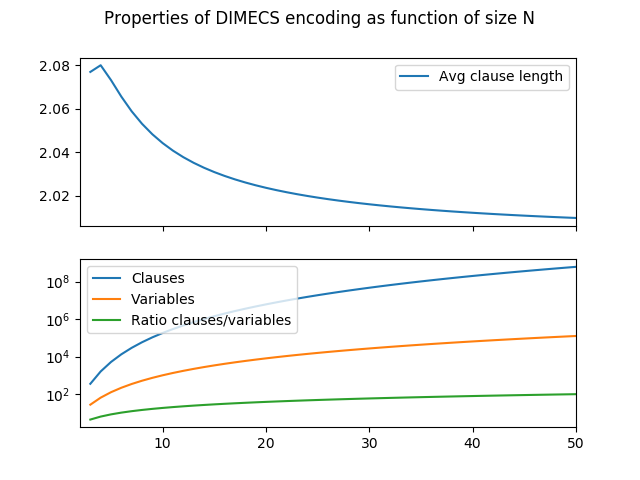
\includegraphics[width=.9\textwidth]{dimecs_props}
  \label{fig_dimecs_props}
  \caption{Properties of DIMECS encoding}
\end{figure}
